\documentclass{article}
\usepackage[margin=2in]{geometry}
\usepackage{parskip}
\usepackage{graphicx}
\usepackage{cite}
\usepackage[compact]{titlesec}
\usepackage{amsthm}
\usepackage{amssymb}
\usepackage{amsmath}
\usepackage{devanagari}

\pagestyle{plain}
\topmargin -0.6in
\textheight 9.5in
\oddsidemargin 0.6in
\textwidth 5in

\title{\textbf{Discovering Lexical Classes and Syntax using Word Embeddings\\ (Report with Annotated Bibliography)}}
\author{\normalsize Pranjal Singh(10327511)\\}

\titleformat*{\section}{\large\bfseries}
\begin{document}
\maketitle
\begin{figure}[h!tb]
\centering

\includegraphics[width=8cm,height=8cm]{6.eps}
\end{figure}
\vspace{5cm}
\begin{center}
\large{
Purpose: M.Tech. Thesis(CS699)\\Semester I(2014-15)\\
Advisor: Prof. Amitabha Mukerjee}
\end{center}
\newpage

\begin{abstract}
Word embeddings have the power to capture semantics.They have potential to represent syntax and semantics both. We have many sources of unsupervised raw data but not supervised data. Unsupervised techniques could greatly improve existing supervised (Collobert et al.(2013)). By leveraging large amount of data floating around, we can improve existing systems. We want to design a framework that will be unsupervised and can induce lexical classes and syntax from the given data by building vector representations, also popularly known as word embeddings.
We may further want to extend this framework for languages such as Hindi which is poor in terms of resources.
\end{abstract}

\section{Problem Statement and Idea}
LSA and LDA were used to capture word embeddings(not exactly) and hence derive semantic relations. Most of the existing systems treat word as atomic units but words also inherit meanings which can only be defined if we represent it as a vector/combination of latent words. So the goal is to maximize probability of raw text given a context window.
So for a given context window of size c:
\begin{center} max $ \frac{1}{T}\sum_{t=1}^T \log p(w_t | w_{t-c}^{t+c}) $  \end{center}

\section{Work Done}
\begin{itemize}
\item Survey of existing literature
\item Ran code provided by Collobert and Weston[9] (SENNA)
\item Buit vector space representation of Hindi words by training on wikipedia dump
\item Derived similar words by using Cosine Similarity technique to create visual embeddings
\end{itemize}

\section{Presentation}
\begin{itemize}
\item Semester presentation\\
\emph{http://home.iitk.ac.in/~spranjal/thesis/bmg\_sem9.pdf}
\end{itemize}

\section{Earlier Work}
This section discusses three important earlier work related to the current work.
\subsection{word2vec}
This work utilized two architectures discussed below:
\subsubsection{CBOW}
Embeddings are represented by a set of latent variables and initialized randomly. Training learns these for each word $w_t$ in the vocabulary.\\
So for a given context window of size c:
\begin{center} max $ \frac{1}{T}\sum_{t=1}^T \log p(w_t | w_{t-c}^{t+c}) $  \end{center}
where
\begin{center} max $ p(w_t | w_{t-c}^{t+c}) = \frac{exp({e'}_{w_t}^{T}.\sum_{-c \leq j \leq c,j\neq 0}e_{w_{t+j}})}{\sum_{w} exp({e'}_{w_t}^{T}.\sum_{-c \leq j \leq c,j\neq 0}e_{w_{t+j}})} $  \end{center}

\subsubsection{Relational Constraint Model}
Define R as a set of relation between two words and relations have scores associated to indicate strength.
\begin{center} max $ \frac{1}{N}\sum_{i=1}^N \sum_{w \in R_{w_i}}\log p(w | w_i) $  \end{center}

\subsection{NLP from Scratch}
This work proposes a unified architecture for NLP tasks such as POS tagging, Chunking, NER and SRL. They have compared against classical NLP benchmarks. The works avoids task specific engineering and generalizes the system to handle multiple tasks.\\
They learn lookup table by back propagation. The words are mapped to d-dimensional vector using lookup table operation. At the end, the lookup table returns a matrix for a given sentence which can be used in training the neural network.\\
They have used entire English Wikipedia to learn word embeddings (631 million words) and they tokenized it using Penn Treebank tokenizer.\\ 
The total training time was about four weeks. The parameters of the model were:\\
Window size: 11 and a Hidden layer with 100 units \\
The objective is to seek a network that computes a higher score when given a legal phrase than when given an incorrect phrase.
\begin{center} $ \theta := \sum_{x \in X} \sum_{w \in D} max \{0,1-f_{\theta}(x)+f_{\theta}(x^{(w)}) \} $  \end{center}
\begin{figure}[h!tb]
\centering
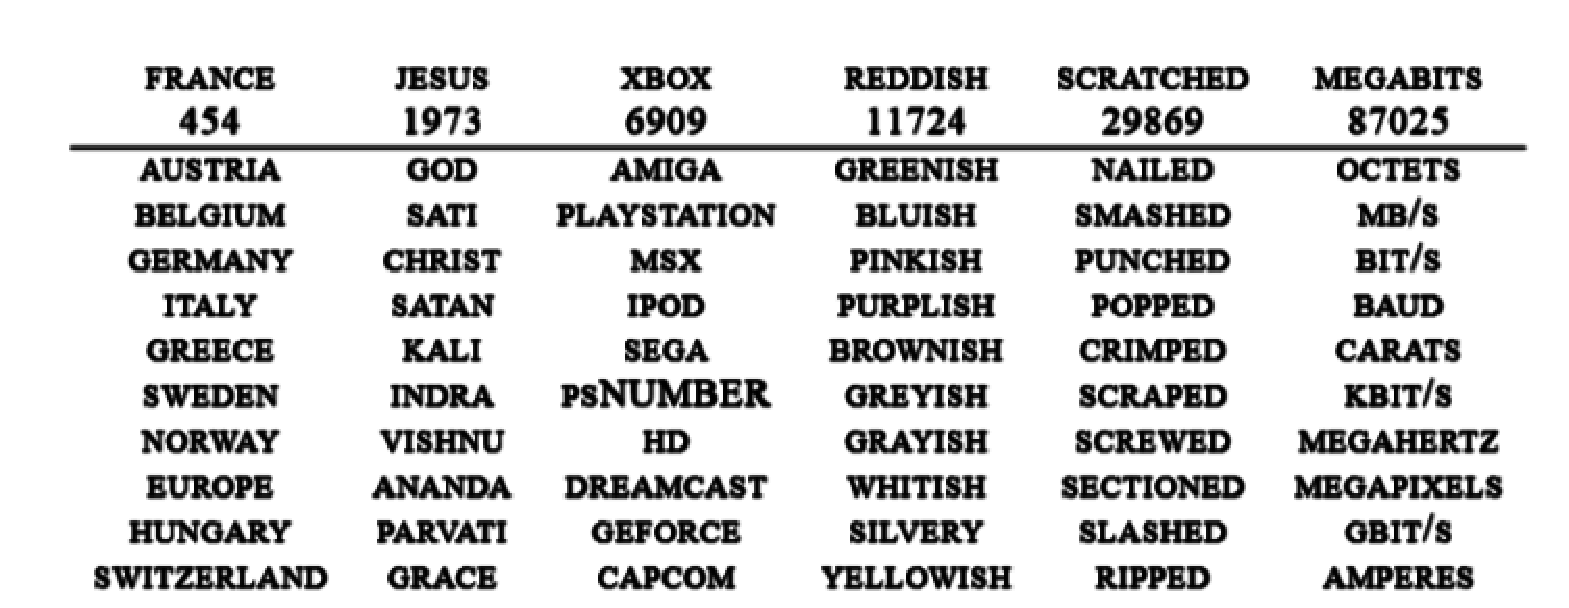
\includegraphics[width=12cm,height=8cm]{5.eps}
\caption {Word Embeddings}
\end{figure}

\subsection{Bilingual Word Embeddings}
It proposes a method to learn bilingual embeddings rather than just monolingual embeddings. So it utilizes counts of Machine Translated alignments derived from Berkeley aligner to initialize monolingual embeddings of another language.
\begin{center} $ W_{t-init}= \sum_{s=1}^{S} \frac{C_{ts}+1}{C_{t}+S}W_{s} $  \end{center}
They have used the same formulation as \emph{Collobert et al.}(2008) to learn embeddings except that they have used global context information as in \emph{Huang et al.}(2012)\\\\
Their objective function captures information of both monolingual embedding and also on translation matrices, also called alignment matrices. They have trained on 100K-vocabulary word embeddings.
With 500,000 iterations it took 19 days of training on 8-core machine. For phrase similarity in 2 languages, they have averaged out the word embedding vectors corresponding to each word in both phrases and then taken cosine similarity to quantize amount of semantic similarity.

\section{Dataset}
\begin{itemize}
\item English wikipedia dump (Size: 95MB)
\item Hindi wikipedia dump (Size: 279MB)
\end{itemize}

\section{Results}

\subsection{English}
\subsubsection{Embeddings}
We find the top 10 embeddings for the word \emph{girl} given below.
\begin{center} \emph{"boy" is to "father" as "girl" is to ...?} \end{center}
\begin{center}
    \begin{tabular}{ | l | l |}
    \hline
    Word & Cosine Similarity  \\ \hline
    Mother & 0.6219688653945923 \\ \hline
    Grandmother & 0.5560075640678406 \\ \hline
    Wife & 0.5442352890968323 \\ \hline
    \end{tabular}
\end{center}
\subsubsection{Similarity}
This experiment finds the most similar word for the query.
\begin{center}
    \begin{tabular}{ | l | l | l | l |}
    \hline
    Given Word11 & Given Word12 & GivenWord21 & FoundWord22  \\ \hline
    he & his & she & \textbf{her} \\ \hline
    big & bigger & bad & \textbf{worse} \\ \hline
    going & went & being & \textbf{were} \\ \hline
    \end{tabular}
\end{center}

\subsubsection{Odd One Out}
This experiment finds the odd word in the provided list.\\\\
\emph{breakfast}
\emph{cereal}
\emph{dinner}
\emph{lunch}
\\\\
\textbf{Result:} \emph{cereal}

\subsection{Hindi}
\subsubsection{Embeddings}
We find the top 10 embeddings for the word \emph{bharat} given below.
\begin{figure}[h!tb]
\centering
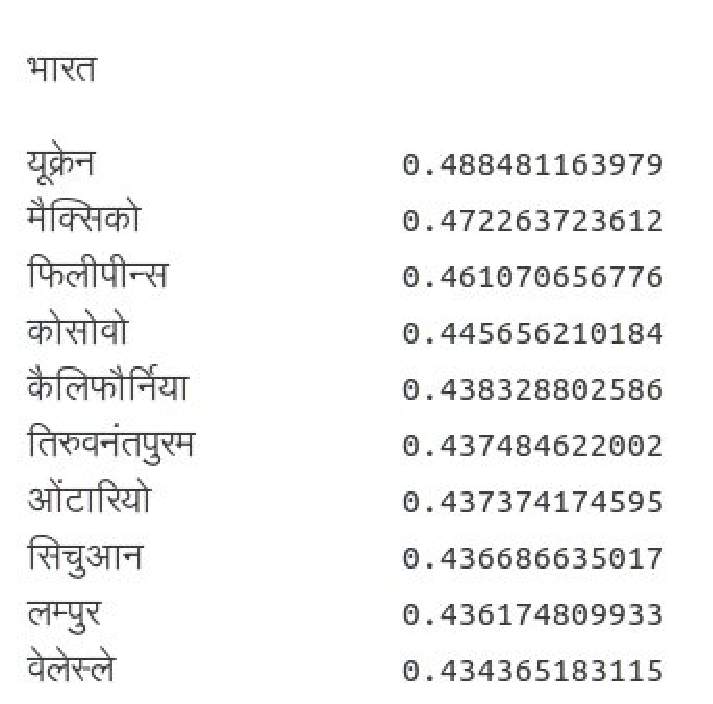
\includegraphics[width=6cm,height=6cm]{1.eps}
\caption {Top few Embeddings in context of another word}
\end{figure}

\begin{figure}[h!tb]
\centering
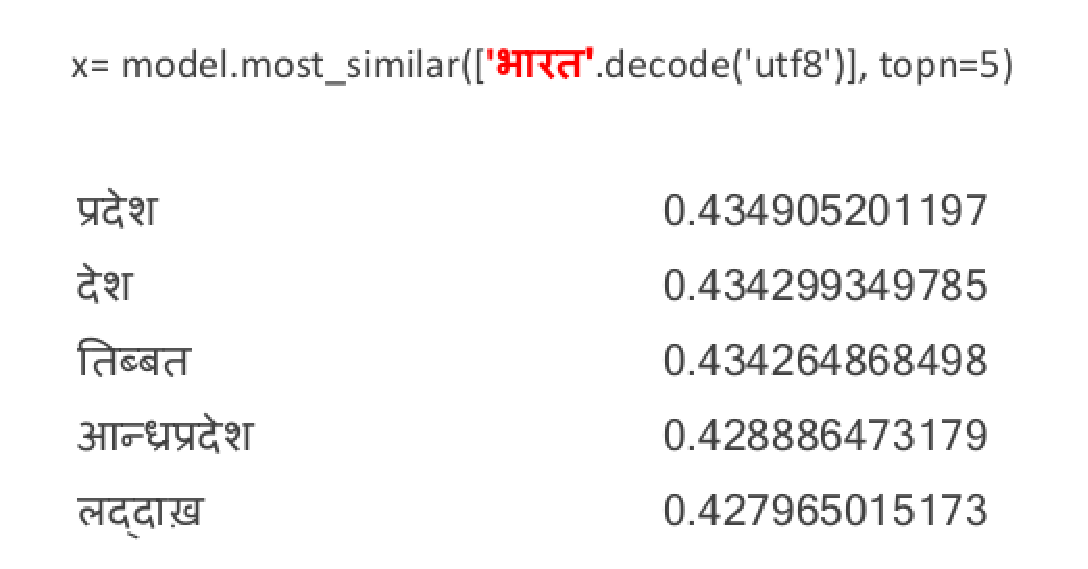
\includegraphics[width=8cm,height=4cm]{3.eps}
\caption {Top 5 embeddings for word \emph{bharat}}
\end{figure}

\begin{figure}[h!tb]
\centering
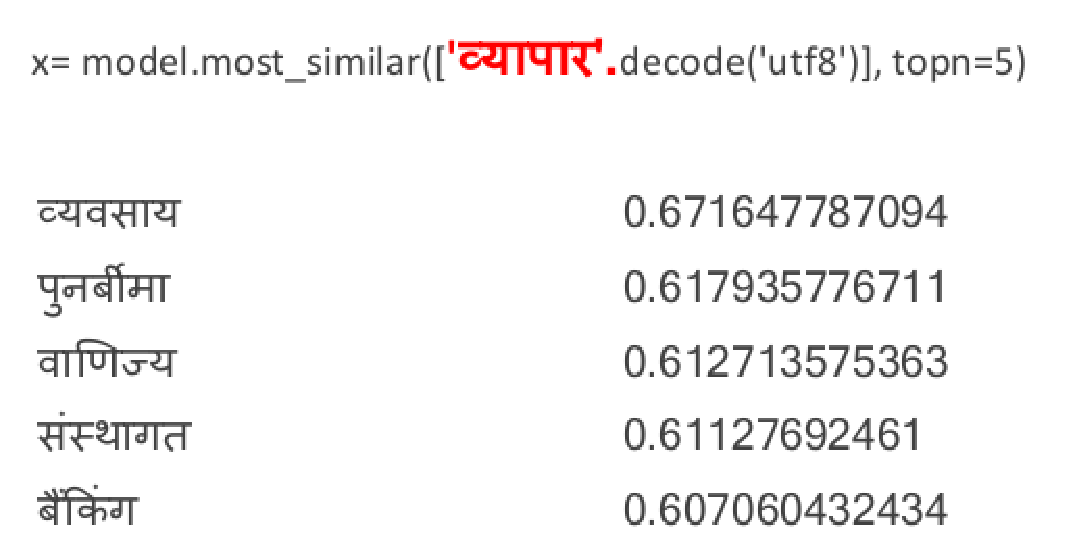
\includegraphics[width=8cm,height=4cm]{4.eps}
\caption {Top 5 embeddings for word \emph{vyapar}}
\end{figure}

\subsubsection{Odd One Out}
This experiment finds the odd word in the provided list.
\begin{figure}[h!tb]
\centering

\includegraphics[width=3cm,height=4cm]{2.eps}
\caption {Blue is the odd one out; Red ones are the queries}
\end{figure}
\newpage

\section{Future Work}
Collobert-Weston claim that their system is generalized for various NLP tasks. This could lead to a big disaster if we use these embeddings for Sentiment Classification task. The current trainig conditions would bring words such as \textbf{good} and \textbf{bad} in close proximity. But they tend to represent opposite poles. This is an open area to extend the work.\\
One exciting think to look at is what if we use these embeddings as functions and operate on other embeddings, e.g., if we ADD the embeddings or if we SUBTRACT the embeddings.
\begin{center}
\emph{Very Big}\\
\emph{Bigger}\\
\end{center}
Such phrases and words should have greater semantic similarity. We could experiment with operations such as addition/subtraction and could get a better insight into such relationships (applicable for Hindi also).

\begin{center}
\emph{Indian Cricketer}\\
\emph{Sachin}\\
\end{center}
Infact above phrase and word may belong to same embedding because they they tend to be very close when it comes to their semantic relationship.\\
The embeddings obtained could help in initializing the embeddings used in work of Collobert and Weston where they suffered problems due to random initialization.\\
\emph{Manning et al.}(2013) have used semantic information to improve word embeddings and \emph{Collobert et al.}(2008) have used large unlabeled data to do the same thing. We could use syntactic or morphological information to improve word embeddings or even produce some good word embeddings. The motivation for this idea could be that morphologically similar words have some sought of close connection between them.\\
e.g. morphology, phonology, etymology
\section{Acknowledgement}
I would like to show my sincere gratitude towards Prof. Amitabha Mukerjee, Computer Science and Engineering Department, IIT Kanpur for his motivation to do this work and becoming my advisor for this work. I would also like to thank my all friends who have helped me throughout this project.
\newpage
\nocite{*}
\bibliography{report}
\bibliographystyle{unsrt-annote}
\end{document}
